\documentclass[a4paper,hidelinks,14pt]{extarticle}

\usepackage[utf8]{inputenc}
\usepackage[T2A]{fontenc}
\usepackage[english, russian]{babel}
\usepackage{lipsum}
\usepackage{amsmath}
\usepackage{amssymb}
\usepackage{amsfonts}
\usepackage{mathtools}
\usepackage{datetime}
\usepackage[pdftex]{graphicx}
\usepackage{indentfirst}
\usepackage{asymptote}
\usepackage{systeme}
\usepackage[dvipsnames]{xcolor}
\usepackage{lastpage}
\usepackage{fancybox,fancyhdr}
\usepackage{hyperref}
\usepackage[font={small,it}]{caption}
\fancyhead[L]{Лабораторная работа №3}
\fancyhead[C]{}
\fancyhead[R]{\textit{Задачи}}
\fancyfoot[L]{}
\fancyfoot[C]{\thepage\space}
\fancyfoot[R]{}
\pagestyle{fancy}
\newcommand{\gt}{\textgreater}
\newcommand{\lt}{\textless}
\usepackage{listings}
\usepackage{xcolor}
\lstset{
    basicstyle=\ttfamily\small,
    keywordstyle=\color{blue},
    commentstyle=\color{gray},
    stringstyle=\color{red},
    numbers=left,
    numberstyle=\color[gray]{0.7}\ttfamily\small,
    stepnumber=1,
    numbersep=8pt,
    frame=single,
    showstringspaces=false,
    tabsize=4,
    breaklines=true
}
\usepackage{subcaption}

\begin{document}
	\section{2D-траектория}
    Требуется синтезировать управление, следящее за синусоидой, амплитуда которой изменяется по гармоническому закону. Пусть это
    \[
        \varphi(x, y) = y - A(x) \sin x = 0, \quad A(x) = 1 + \cos(2 x)
    \]

    При этом параметры системы (масса и момент инерции):
    \[
        m = 1.2, \quad J = 1
    \]

    Начальные условия (положение и ориентация):
    \[
        (x_0, y_0) = (0, 1.5), \quad \alpha_0 = \pi/4
    \]

    Желаемая скорость $s^* = 1$, а коэффициенты регулятора:
    \[
        k_s = 10, \quad k_{e1} = k_{e2} = 20, \quad k_{d1} = k_{d2} = 40
    \]

    Результаты моделирования представлены на рисунках \ref{fig:track2d} и \ref{fig:errors2d}. Видим, что ошибки ограничены, но не сходятся в ноль.
    \begin{figure}
        \centering
        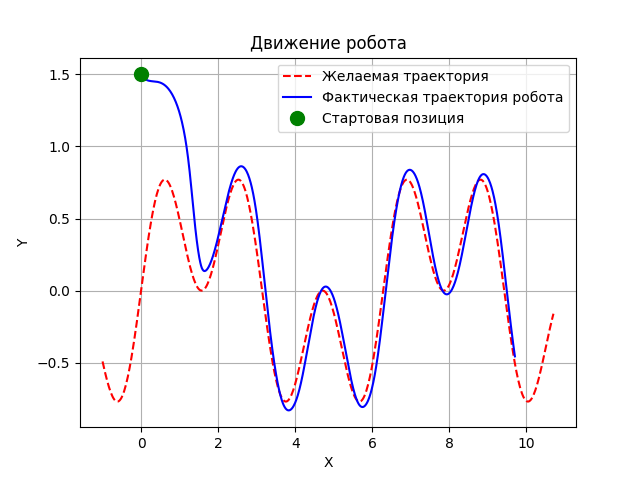
\includegraphics[width=0.8\textwidth]{track2d.png}
        \caption{Слежение за траекторией $\varphi(x, y) = 0$ при $s^* = 1$}
        \label{fig:track2d}
    \end{figure}
    \begin{figure}
        \centering
        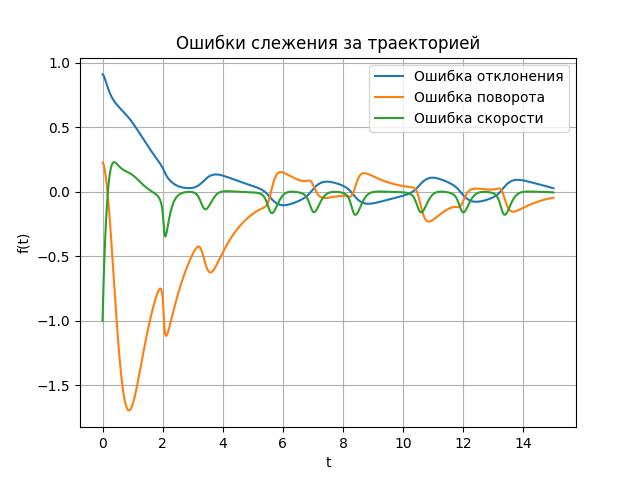
\includegraphics[width=0.8\textwidth]{errors.png}
        \caption{Ошибки слежения за траекторией $\varphi(x, y) = 0$ при $s^* = 1$}
        \label{fig:errors2d}
    \end{figure}
    \begin{figure}
        \centering
        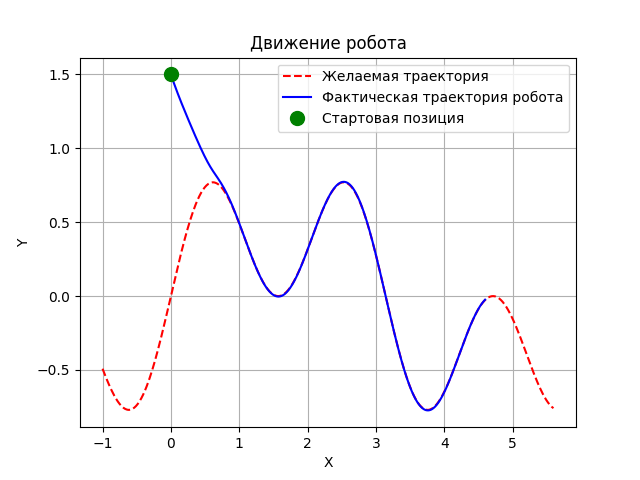
\includegraphics[width=0.8\textwidth]{track2d_s.png}
        \caption{Слежение за траекторией $\varphi(x, y) = 0$ при $s^* = 0.1$}
        \label{fig:track2d_s}
    \end{figure}
    \begin{figure}
        \centering
        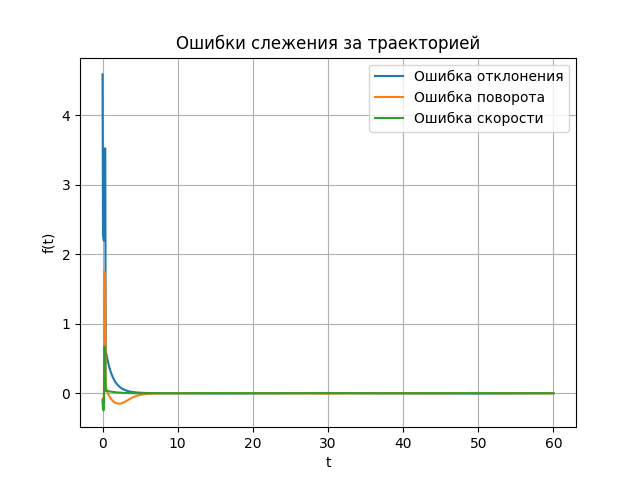
\includegraphics[width=0.8\textwidth]{errors_s.png}
        \caption{Ошибки слежения за траекторией $\varphi(x, y) = 0$ при $s^* = 0.1$}
        \label{fig:errors2d_s}
    \end{figure}

    Уменьшение желаемой скорости до $s^* = 0.1$ (в десять раз) сильно улучшает качество слежения, сводя ошибки ближе к нулю, однако движение при этом медлительно (в связи с чем пришлось увеличить и время моделирования). Результаты при $s^* = 0.1$ отображены на рисунках \ref{fig:track2d_s} и \ref{fig:errors2d_s}.

    \newpage

    \section{3D-траектория}
    Требуется синтезировать управление, следящее за винтовой траекторией, заданной на цилиндре, то есть желаемое движение задаётся через пересечение двух уравнений ($R = 15$)
    \[
        \varphi_1(x, y, z) = x^2 + y^2 - R^2 = 0, \quad \varphi_2(x, y, z) = z - p \theta(x, y, z) = 0
    \]

    Здесь $p = 5$ - шаг винта, а $k$ - вспомогательный параметр, определяющий, на каком номере ветка должен находиться робот. Параметр $k$ необходим, чтобы робот не срывался с траектории на веток выше или ниже:
    \[
        \theta(x, y, z) = \text{atan2}(y, x) + 2\pi k, \quad k = \text{round}\left( \frac{z/p - \text{atan2}(y, x)}{2\pi} \right)
    \]

    При этом параметры системы (масса и инерция):
    \[
        m = 1.2, \quad J = I
    \]

    Начальные условия (положение и ориентация):
    \[
        (x_0, y_0, z_0) = (18, 2, -10), \quad n_0 = \begin{bmatrix}
            1 & 1 & 0
        \end{bmatrix}/\sqrt{2}
    \]

    Желаемые скорость и ориентация:
    \[
        s^* = 3, \quad n_d = \begin{bmatrix}
            1 & 1 & 1
        \end{bmatrix}/\sqrt{3}
    \]

    Результаты моделирования представлены на рисунках \ref{fig:trajectory_3d} и \ref{fig:position_error}. Видим, что слежение успешно выполняется - регулятор справляется с поставленной задачей.
    \begin{figure}
        \centering
        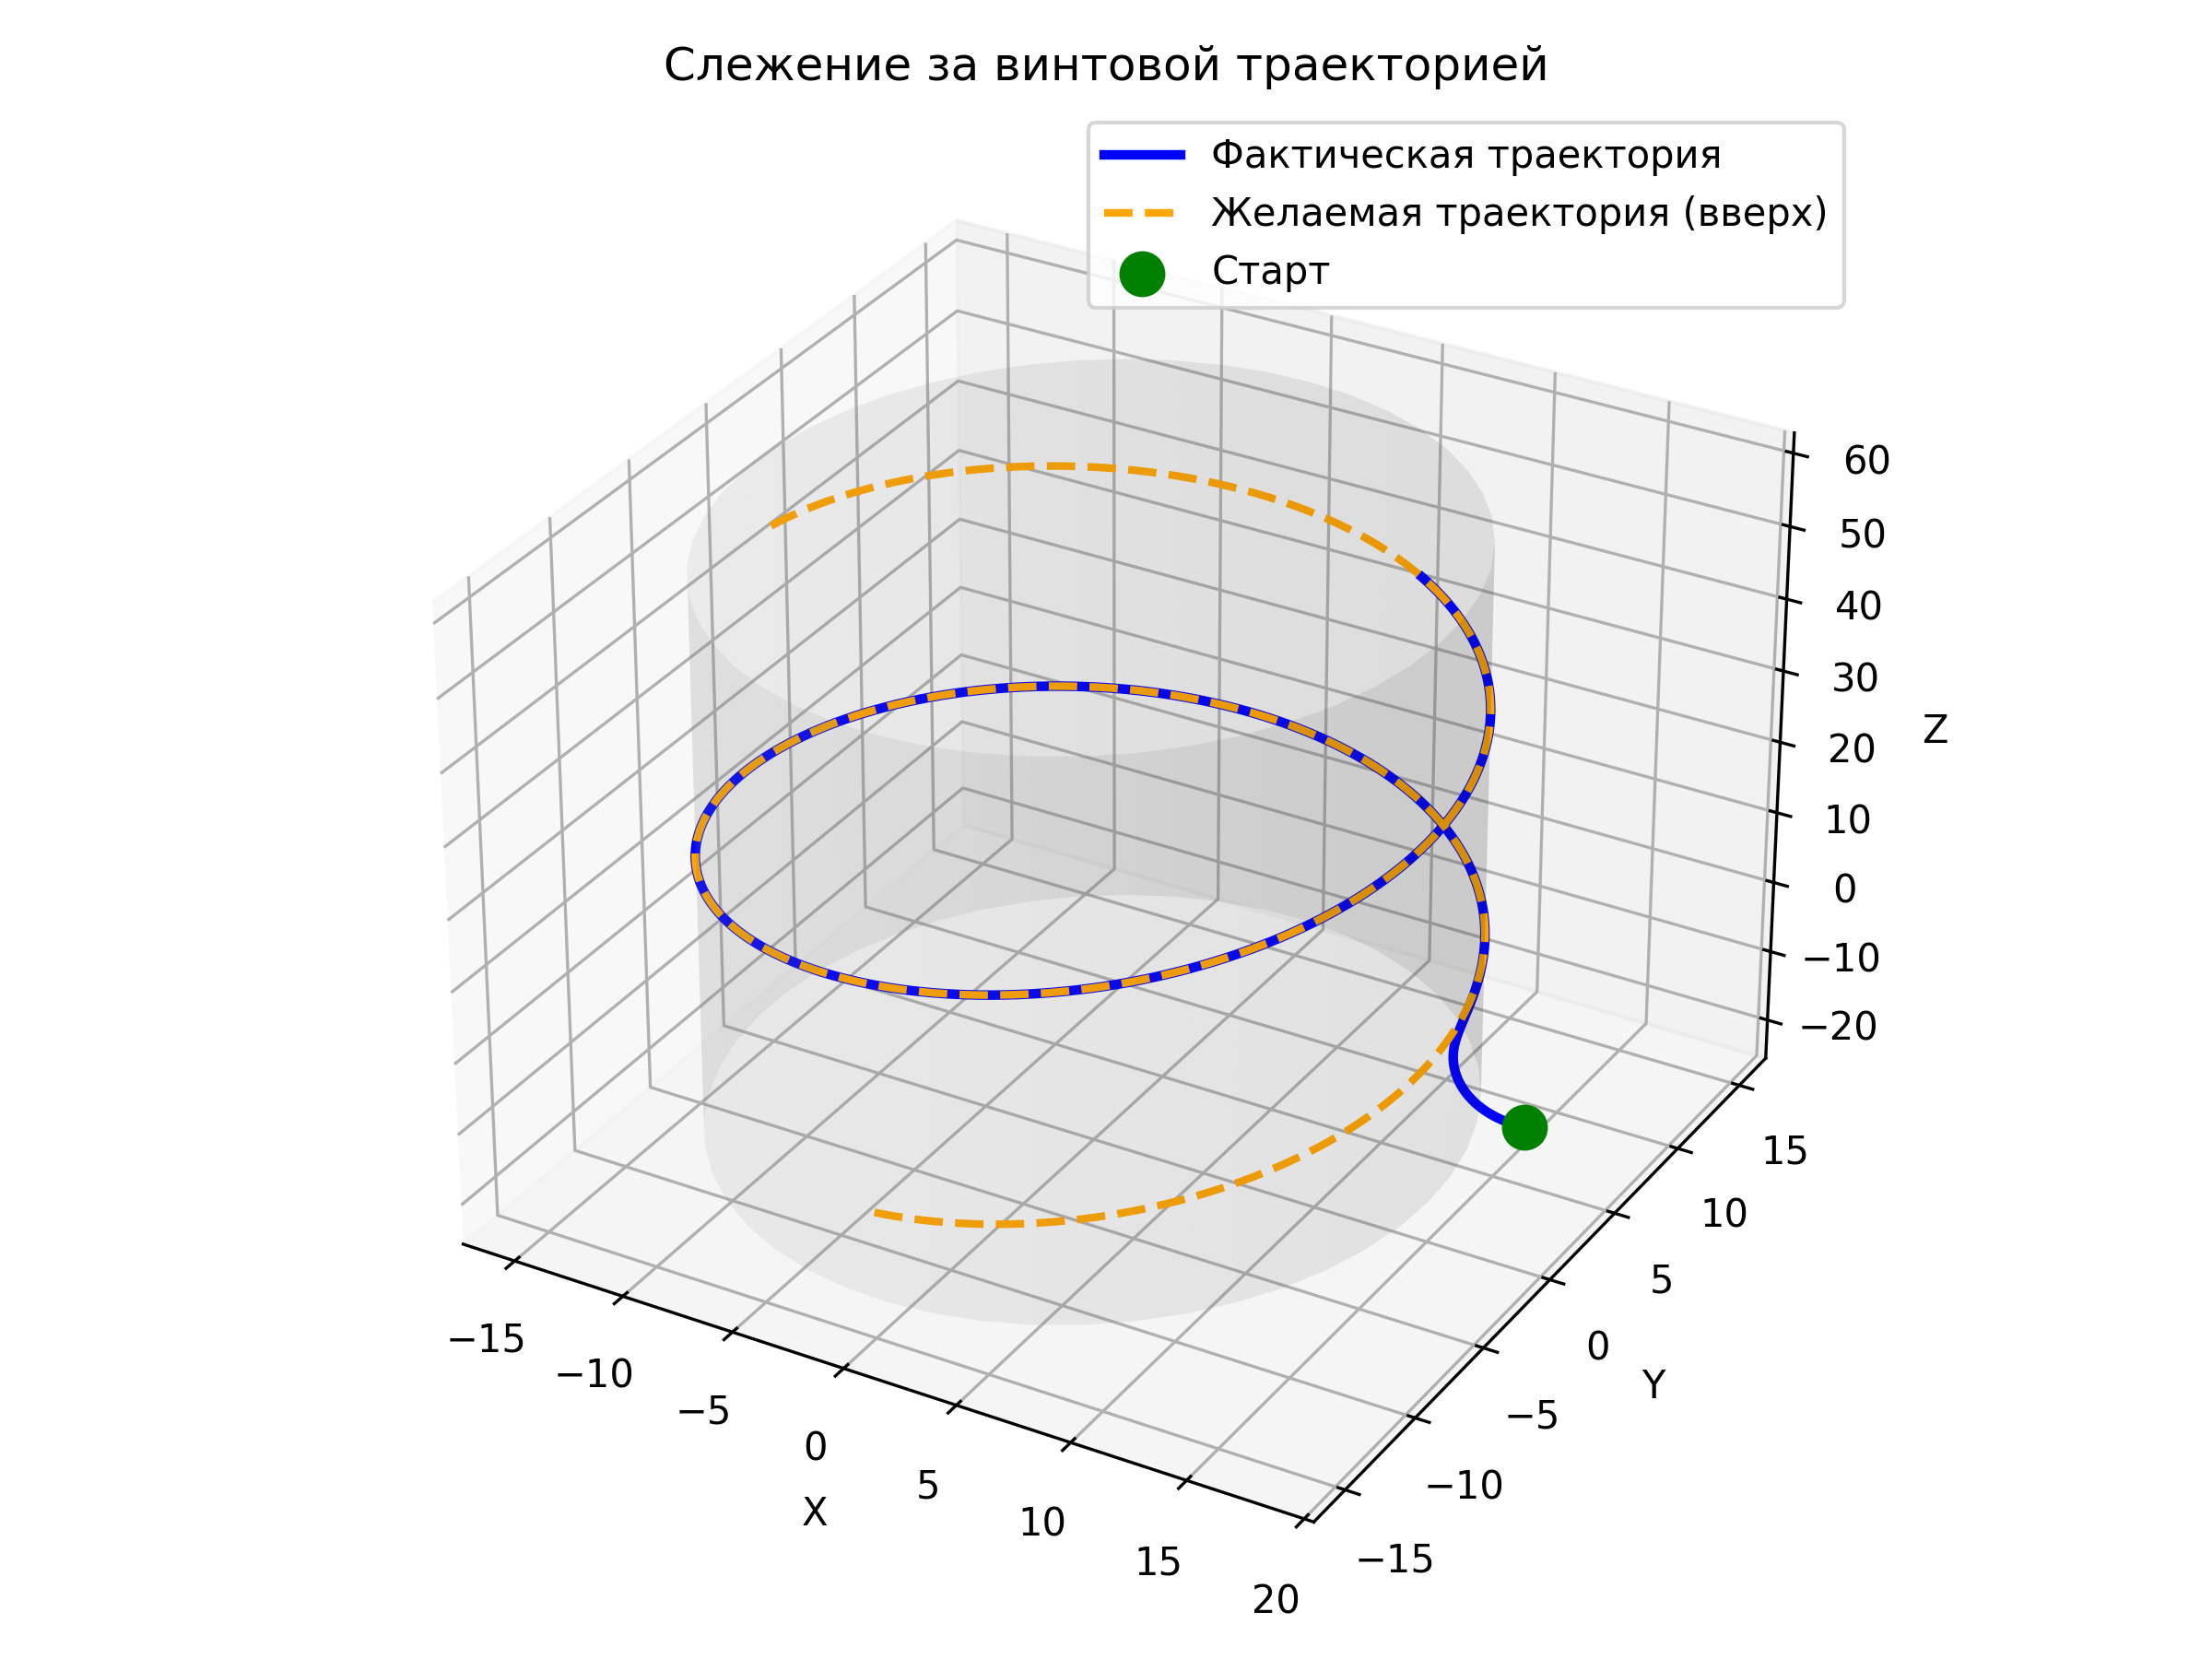
\includegraphics[width=0.8\textwidth]{trajectory_3d.png}
        \caption{Ошибки слежения за траекторией $\varphi_1(x, y, z) \cap \varphi_2(x, y, z) = 0$}
        \label{fig:trajectory_3d}
    \end{figure}
    \begin{figure}
        \centering
        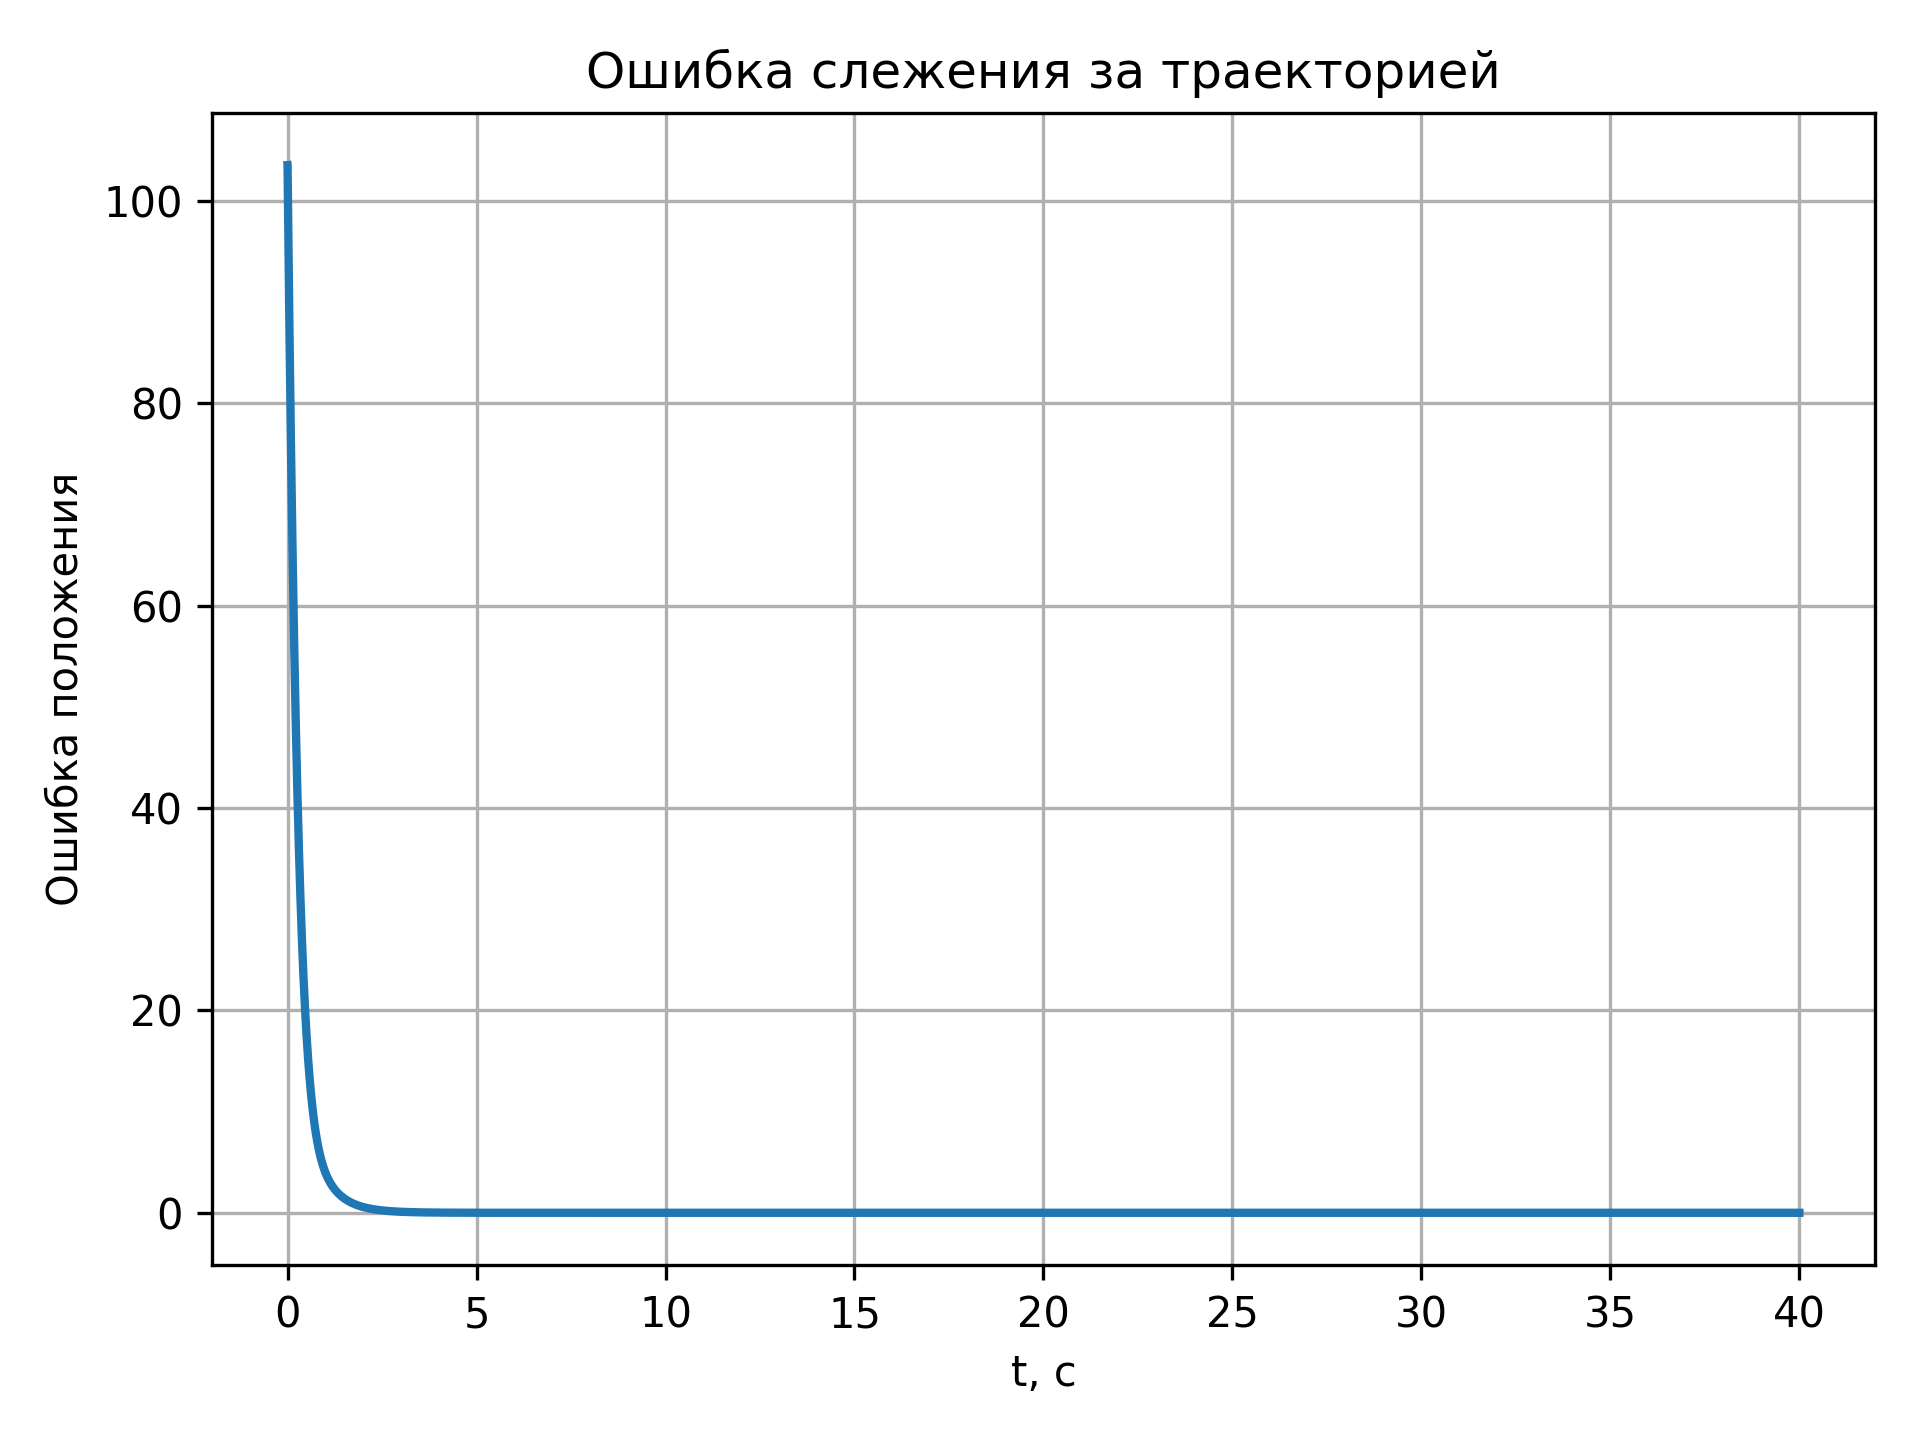
\includegraphics[width=0.8\textwidth]{position_error.png}
        \caption{Ошибка положения при слежении за траекторией $\varphi_1 \cap \varphi_2 = 0$}
        \label{fig:position_error}
    \end{figure}

    При этом ошибка по положению была вычислена из:
    \[
        e_1 = \varphi_1(x, y, z), \quad e_2 = \varphi_2(x, y, z)
    \]
    \[
        e = \sqrt{e_1^2 + e_2^2}
    \]




    
    



	

	


\end{document}